\section{Sensoren}

\subsection{Neo 7M}
Das Neo 7m Modul ist ein sehr kleiner GPS-Sensor, welcher mittels einer Antenne die eigenen GPS-Koordinaten auslesen kann. Es wird in unserem Fall über eine UART-Schnittstelle angesteuert. \\
\\
Die Genauigkeit ist leider stark abhängig vom Gelände, dem Wetter und ob die Antenne “Sichtkontakt” zum Himmel hat. Ausserdem wird der Empfang von GPS-Koordinaten nicht funktionieren, wenn das Modul sich nicht unter freiem Himmel befindet.

\begin{figure}[H]
    \begin{center}
    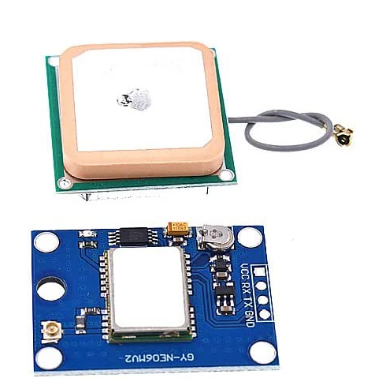
\includegraphics[height=4cm]{Sensoren_Neo 7M.png}
    \end{center}
    \caption{GPS Modul}
\end{figure}

\subsection{QMC5883L}
Das QMC5883 Kompass Modul ist ein Magnetometer, welches mit der richtigen Bibliothek in der Lage ist, einen Kompass zu simulieren. So können Azimut und Himmelsrichtungen direkt ausgelesen werden. Es ist allerdings Vorsicht geboten, der Kompass ist sehr empfindlich auf Magnetismen und Metalle. Derartige Einflüsse können die Zuverlässigkeit der Daten des Kompasses stark beeinflussen.

\begin{figure}[H]
    \begin{center}
    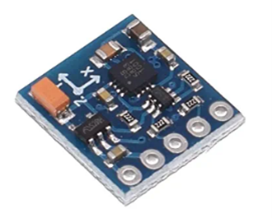
\includegraphics[width=3.2cm]{Sensoren_Kompass.png}
    \end{center}
    \caption{Kompass Modul}
\end{figure}

\pagebreak

\subsection{HC-05}
Das HC-05 ist ein Bluetooth-Modul mit sowohl Slave- als auch Master Fähigkeiten. Es soll die Kommunikation/Datenübertragung zwischen dem Handy und dem Arduino ermöglichen. 

\begin{figure}[H]
    \begin{center}
    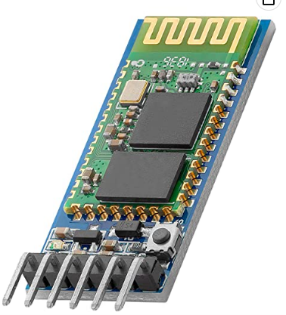
\includegraphics[width=3.3cm]{Sensoren_Bluetooth Modul.png}
    \end{center}
    \caption{Bluetooth Modul}
\end{figure}

